\begin{table}[ht]
    \centering
    \begin{tabular}{l|lrr}
        \textbf{Developer} & \textbf{Model} & \textbf{\#Param} & \textbf{\$ per M/Tok} \\
        \hline
        OpenAI  & gpt-3.5-turbo     & ${\dagger}$ & 00.50/01.50 \\
        ~       & gpt-4             & ${\dagger}$ & 30.00/60.00 \\
        ~       & gpt-4-turbo       & ${\dagger}$ & 10.00/30.00 \\
        ~       & gpt-4o           & ${\dagger}$ & 05.00/15.00 \\
        ~       & ~                 & ~             & ~     \\
        Google  & gemini-1.0-pro    & ${\dagger}$ & 00.50/01.50 \\
        ~       & gemini-1.5-flash  & ${\dagger}$ & 00.35/01.05 \\
        ~       & gemini-1.5-pro    & ${\dagger}$ & 03.50/10.50 \\
        ~       & ~                 & ~             & ~     \\
        Anthropic & claude-3-opus & ${\dagger}$ & 15.00/75.00 \\
        ~       & claude-3-sonnet & ${\dagger}$ & 03.00/15.00 \\
        ~       & claude-3-haiku & ${\dagger}$ & 00.25/01.25 \\
        ~       & ~                         & ~             & ~      \\
        Meta    & llama3-70b        & 70b       & 03.20/03.20 \\
        ~       & llama3-8b         & 8b        & 01.60/01.60 \\
        ~       & ~                         & ~             & ~      \\
        Mistral & mixtral-8x22b-instruct & 39b/141b  & 03.20/03.20 \\
        ~       & mistral-7b-instruct & 7b     & 01.60/01.60 \\
    \end{tabular}
    \caption{Summary of models evaluated.${\dagger}$ denotes where information has not been publicly disclosed.}
    \label{tab:models}
\end{table}

\section{Results}
\label{section:results}

In this section we discuss the results of the experiments described in the previous section.

\subsection{Result 1. Toponym Resolution}

\begin{figure}
    \centering
    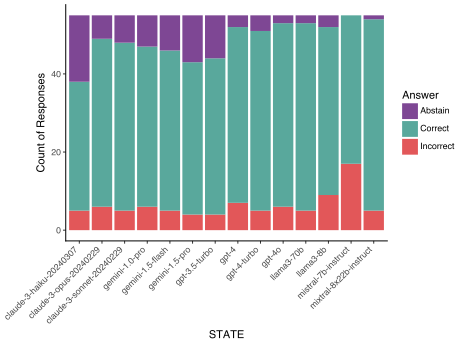
\includegraphics[width=\columnwidth]{figures/toponym_bar_state}
    \caption{The results of the toponym experiments show that most models resolve most toponyms to Australia. }
    %We filter out the `confusing' toponyms for subsequent experiments}
    \label{fig:toponym}
\end{figure}

The toponym experiments shown in figure~\ref{fig:toponym} show percentage of responses that were correct, incorrect and abstain. 
Most models are capable of answering toponym resolution questions, with the majority of abstains associated with the less popular or Indigenous place names. 
Mistral-7b produced excessive tokens when answering questions, contributing to its increased error rate, whereas gpt-4 resolved toponyms like `Port Arthur', `Exmouth' and `Roma' to Texas, the United Kingdom and Italy respectively.
These are valid resolutions, but could cause cause correct spatial reasoning to be marked incorrectly, if the model is considering different locations to what the question intended.
To avoid this issue, we ensure than none of the toponyms marked incorrectly in toponym resolution appear together in questions, so that the models should infer the correct resolution given the context of other toponyms resolved to Australia.
% were useful for identifying places that may induce unnecessary friction in subsequent tasks.

% \subsection{R2. Lesser-known Cities}
% --> Show correlation between cities recognized and their population size. Plot for each population value tested the binary value indicating if it was recognized or not by Chat-GPT.
% Give the phrase Chat-GPT outputs when a location is not recognized.
% Plot accuracy of result vs. population size.
%\osullikomment{I think you might get some intersting outliers. E.g. I think Port Arthur will be massively over-represented because it was the site of our last mass shooting, and the catalyst for gun control in Australia. So there are a million articles that talk about Port Arthur, even though it's tiny in real terms.}



\subsection{Result 2. Directional Relationships}
The results for the $22$ 2-way directional prompts in figure~\ref{fig:direcional-2} varied across the models, with \texttt{claude-haiku} unable to answer any question and \texttt{mistral-7b} again struggling because of token over-generation. 
The tests for the $20$ 3-way prompts summarized in Figure~\ref{fig:directional-3} shows that half of the models tested showed a significant increase in model abstention and error rate as compared to the 2-way directional prompts.
For comparison, \citeauthor{Qi2023} performed 2-way directional prompting for major cities in Australia and found the responses to be correct in 44 out of 50 cases~\cite{Qi2023}.


\begin{figure*}[ht]
    \centering
    \begin{subfigure}[Model performance on 2-way directional relation prompts. Results indicate better performance by gpt family of models compared to the other models tested.]{
        % \centering
        \includesvg[width=\columnwidth]{figures/directional_bar_2-way}
        \label{fig:direcional-2}
        }
    \end{subfigure}
    \hfill
    \begin{subfigure}[Model performance on 3-way directional relation prompts. A third constraint decreases answer confidence and accuracy. Gpt models still outperform others, but at a much lower rate of success.]{
        % \centering
        \includesvg[width=\columnwidth]{figures/directional_bar_3-way}
        \label{fig:directional-3}
        }
    \end{subfigure}
    \caption{Results of two directional relation prompts: 2-way and 3-way. Adding a third directional constraint reduces model performance, and also decreases the chance that the question was observed in an LLM's training data.}
    \label{fig:directional}
\end{figure*}



\subsection{Result 3. Topological Relationships}

\begin{figure*}[h]
    \centering
    \subfigure[Performance on topological questions containing line entities asking about `intersect' relationship. High error-rates are observed for several OpenAI, Google, and Anthropic models, while Meta models perform well.]{
        \includesvg[width=0.3\textwidth]{figures/topological_bar_intersect_line-line}
        \label{fig:topo-intersect}
    }
    \hfill
    \subfigure[Performance on topological questions asking about `partial overlap' relationship. Models abstain from answering a consistently high proportion of the questions.]{
        \includesvg[width=0.3\textwidth]{figures/topological_bar_Partially Overlap_region-region}
        \label{fig:topo_overlap}
    }
    \hfill
    \subfigure[Performance on topological questions asking about `within' relationship. Models perform consistently well.]{
        \includesvg[width=0.3\textwidth]{figures/topological_bar_within_region-region}
        \label{fig:topo_within}
    }
    \caption{Detailed results for topological reasoning on a selection of entity and relationship types.}
    \label{fig:topo_plots}
\end{figure*}

The performance on topological queries was generally stronger than other relation types, but as figure~\ref{fig:topo-intersect} shows, line-based relations tend to have a higher error rate. 
We expect that the higher error rate is because of reduced presence of these terms in the training corpus as they relate to each other. 
We observe in figure~\ref{fig:topo_overlap} that uncertainty rises when, when there are multiple possible answers, or multiple constraints are imposed simultaneously imposed. Partial Overlap relations are primarily border-regions and introduce uncertainty about ownership, which is reflected in the higher-than-average abstention rate across all models.
WITHIN: with the only error for gpt-3.5-turbo coming from a question about whether Canberra is within the state of New South Wales (NSW), which is tricky because they are disjoint but NSW surrounds ACT, which contains Canberra. The physical sense contradicts the political in this instance, highlighting some of the reasoning difficulties faced in geospatial computing.

Our system prompt explicitly gives permission to not answer, and more work is needed to probe how that answerability decision is reached, and why uncertainty triggers it. 
We hypothesize that the better performance on topological relations in general, compared to cyclic order or directional relations is due to two factors.
The first factor is the qualitative nature of topological relations, which lend themselves well to natural language descriptions, making them more prevalent (at least explicitly) in LLM training data.
The second factor is that this test only involved two entities per prompt, which makes it more likely that the information required to answer the question may have been seen explicitly at training time, reducing the need for the model to perform spatial reasoning to answer the question correctly.
%To disentangle these factors, further investigation could be done testing complex topological relations between more than two entities.



\subsection{Result 4. Order Relationships}

\begin{figure}
    \centering
    \includesvg[width=\columnwidth]{figures/order_bar}
    \caption{Summary of results for cyclic order reasoning. Models perform poorly across the board, with some answering every question incorrectly.}
    \label{fig:order}
\end{figure}

The returned results for the cyclic order relation prompts (figure~\ref{fig:order}) show performance on par with or worse than random guessing between `clockwise' and `counterclockwise' by the models.
%In this case, where it is evident that the problem was not within the capability of the models, the decision to abstain appears wise, and note that 
Across the experiments the Google and Anthropic models consistently abstained at higher rates than the other models, which guessed incorrectly for most of the questions.
%Being able to effectively identify when a question cannot be answered is useful and could lead to better reliability of models in future. 











% Report percent of 2 hop spatial queries correct.
% Report percent of space + time queries correct.
% Report for more hops if tested.